\documentclass[11pt]{amsart}
\usepackage{geometry}                % See geometry.pdf to learn the layout options. There are lots.
\geometry{letterpaper}                   % ... or a4paper or a5paper or ... 
%\geometry{landscape}                % Activate for for rotated page geometry
%\usepackage[parfill]{parskip}    % Activate to begin paragraphs with an empty line rather than an indent
\usepackage{graphicx}
\usepackage{amssymb}
\usepackage{epstopdf}
\usepackage{tikz}
\usetikzlibrary{3d,shapes,snakes,positioning}
\DeclareGraphicsRule{.tif}{png}{.png}{`convert #1 `dirname #1`/`basename #1 .tif`.png}

\begin{document}





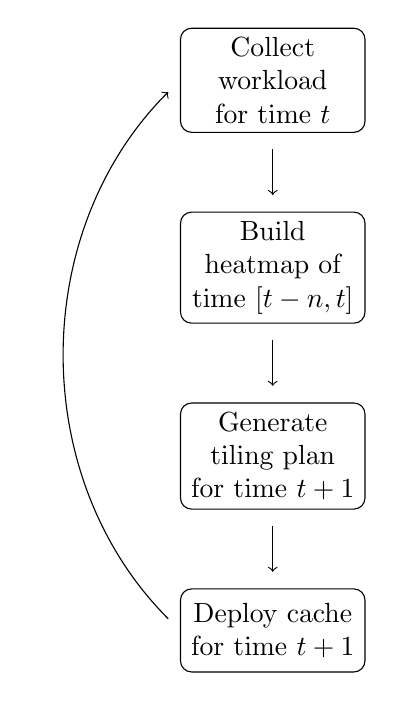
\begin{tikzpicture}[node distance=1cm, auto]

\tikzstyle{kasse}=[rectangle, rounded corners, draw=black, text width=6em, minimum height=3em, text centered]
\tikzstyle{pil}=[->, shorten >=6pt, shorten <=6pt]


\node[kasse] (collect) {Collect workload for time $t$};
\node[kasse, below=of collect] (track) {Build heatmap of time $\lbrack t-n, t \rbrack$};
\node[kasse, below=of track] (predict) {Generate tiling plan for time $t+1$};
\node[kasse, below=of predict] (deploy) {Deploy cache for time $t+1$};

\draw[pil] (collect.south) to (track.north);
\draw[pil] (track.south) to (predict.north);
\draw[pil] (predict.south) to (deploy.north);
\draw[pil, bend left=45] (deploy.west) to (collect.west);

\end{tikzpicture}

\end{document}  